Апробация результатов расчетов производилась на лабораторном источнике
рентгеновского излучения (рис. \ref{ris:trs}). Трехкристальный рентгеновский
спектрометр (ТРС) представляет из себя источник с молибденовым анодом, который является
неподвижным в процессе сканирования. Рентгеновские лучи от источника падают на
 кристалл монохроматор, где происходит выделение спектрального дублета. Щелевое
 устройство № 1 отделяет спектральную составляющую, котороя затем отражается от
 исследуемого кристалла.

\begin{figure}[H]
  \centering
  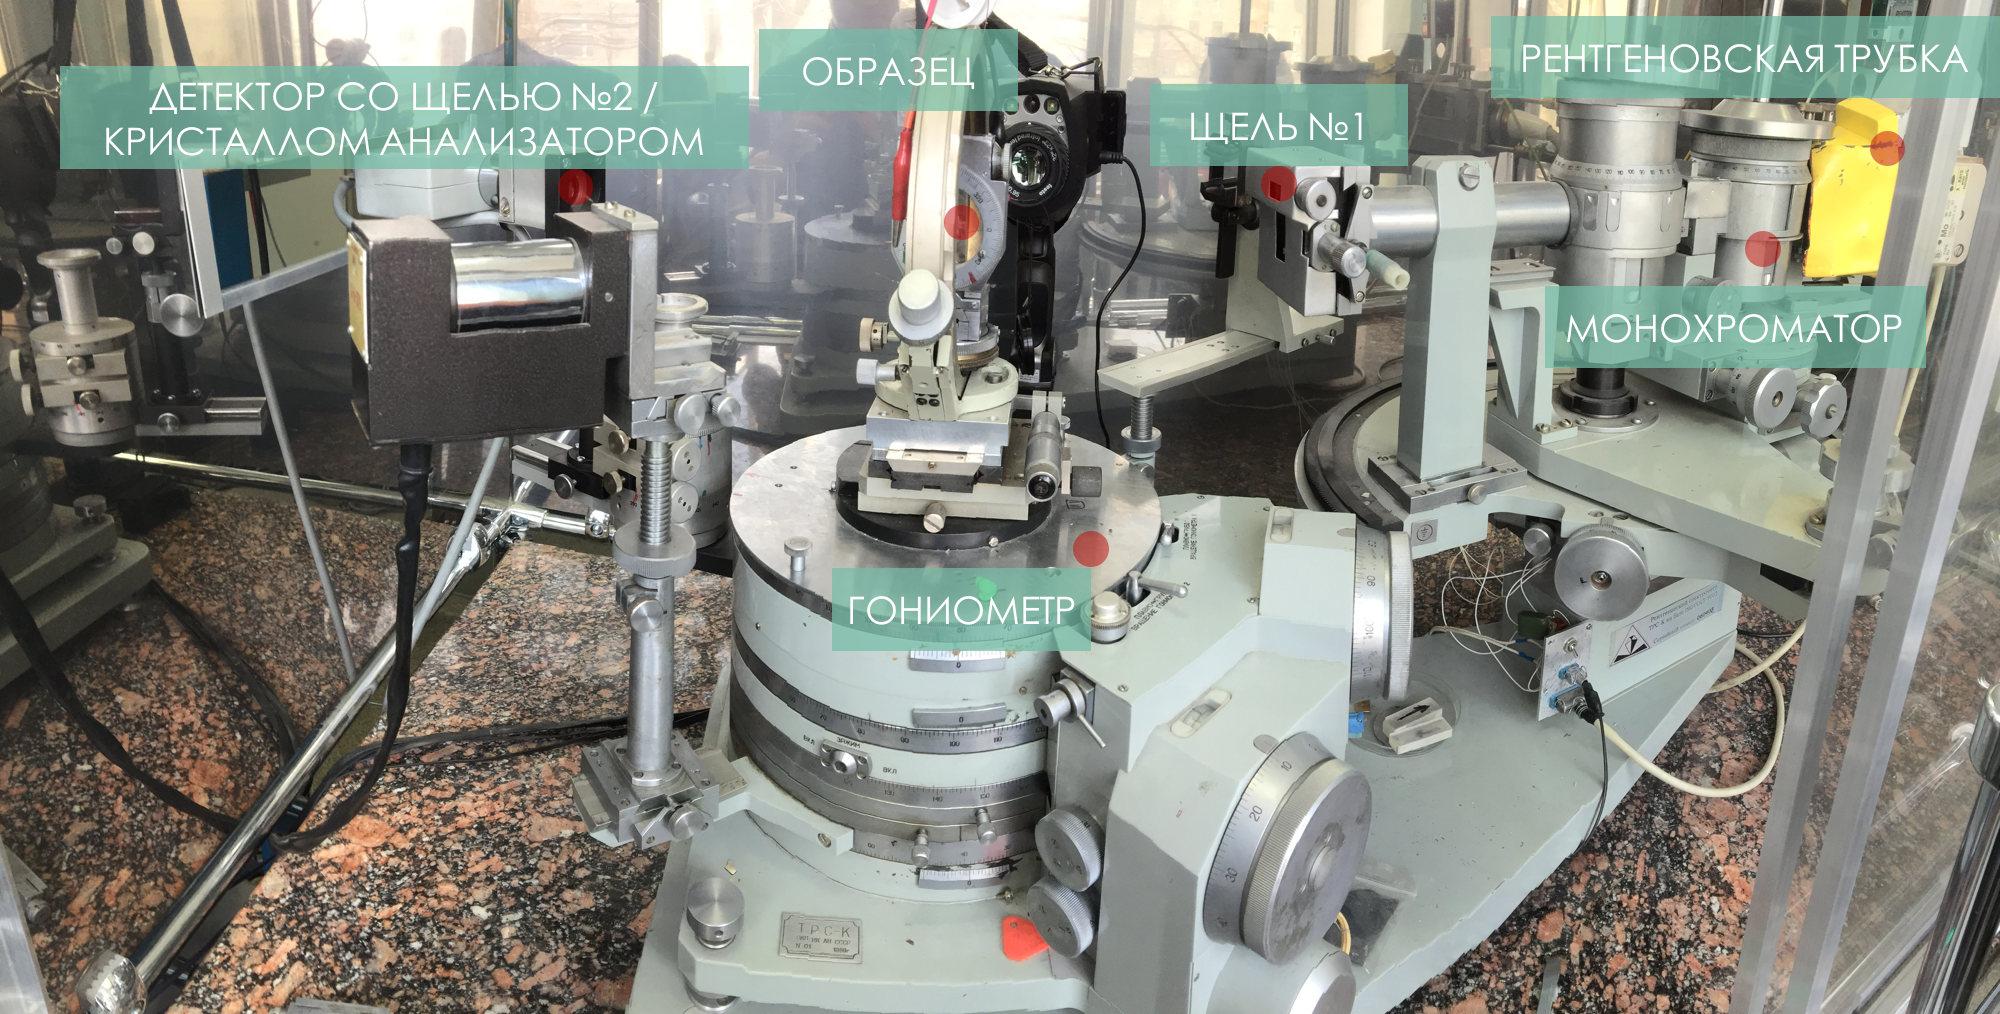
\includegraphics[width=1\textwidth]{images/trs.png}
  \caption{ Трехкристальный рентгеновский спектрометр. Лаборатория рентгеновских
  методов анализа и синхратронного излучения, ФНИЦ "Кристаллография и фотоника"}
  \label{ris:trs}
\end{figure}

ТРС имеет возможность работать в режиме двухкристального эксперимента,
в таком случае непосредственно перед детектором устанавливается щелевое устройство
№ 2, все прошедшие лучи фиксируются детектором.

Для случая необходимости получения трехкристальных кривых дифракционного отражения,
на место перед детектором устанавливается кристалл анализатор, отраженный от анализатора луч
фиксируется детектором.
